%-----------------------------------------------------------------------------%
\chapter{\babEmpat}
%-----------------------------------------------------------------------------%


%-----------------------------------------------------------------------------%
\section{Analisis}
\label{sec:analysis}
%-----------------------------------------------------------------------------%
Pada kondisi saat ini, alokasi petugas pengumpulan data di BPS dilakukan pada saat perancangan. Sebelum proses pengumpulan data dilakukan, dan lokasi pencacahan telah diketahui (berdasarkan metode sampling yang digunakan), petugas direkrut dan kemudian dialokasikan kepada lokasi pencacahan terdekat. Pengalokasian lokasi pencacahan terhadap masing-masing pencacah, seringkali dilakukan secara subyektif, akibatnya selain variasi waktu penyelesaian tinggi, juga terkadang menyebabkan ketidakmerataan beban. 


Metode MTSP dan VRP serta berbagai variasinya dapat digunakan untuk mengatasi pengalokasian diatas. Variasi MTSP yang dapat digunakan dalam permasalahan ini antara lain: 

\begin{itemize}
\item Menggunakan lebih dari satu pencacah, dimana masing-masing pencacah memulai dari \textit{depot} yang berbeda-beda;
\item Penimbang dari setiap lokasi pencacahan dengan lokasi lainnya direpresentasikan dengan waktu tempuh. Waktu tempuh lebih representatif untuk digunakan sebagai penimbang dibanding jarak, karena jarak tidak memperhitungkan kesulitan akses.
\end{itemize}


Untuk menggambarkan bagaimana MTSP dapat digunakan untuk mengatasi masalah ini, maka perlu dilakukan eksperimen. Eksperimen ini menggunakan 182 lokasi pencacahan yang merepresentasikan \textit{customer} dalam MTSP, 15 pencacah yang merepresentasikan \textit{salesman}, dan 15 \textit{depot}. Langkah-langkah yang dilakukan dalam eksprerimen adalah sebagai berikut:


%-----------------------------------------------------------------------------%
\subsection{Dataset}
\label{ssec:mtsp_dataset}
%-----------------------------------------------------------------------------%
\subsubsection{Lokasi Pencacahan}
%-----------------------------------------------------------------------------%
Data lokasi pencacahan yang digunakan sebanyak 182 lokasi, yang diambil dari lokasi nagari/kelurahan di Kab. Pesisir Selatan, Sumatera Barat. Masing-masing lokasi dilengkapi atribut ID, sumbu lintang dan sumbu bujur, sebagaimana contoh data yang yang terdapat pada Tabel \ref{tbl:enumeration_locations}. Adapun data lokasi secara lengkap terdapat pada Lampiran \ref{tbl:enumeration_locations_full}.


\begin{table*}
	\centering
	\ra{1.3}
	\caption{Lokasi Pencacahan}
	\label{tbl:enumeration_locations}
	\begin{tabular}{lcc}
		\toprule
			& \multicolumn{2}{c}{Koordinat}\\
		\cmidrule{2-3}
			& Latitude & Longitude\\ 
		\midrule
			1302011001 & -2.3504 & 101.1434\\ 
			1302011002 & -2.4233 & 101.0285\\ 
			1302011003 & -2.3798 & 101.0427\\ 
			1302011004 & -2.3884 & 101.049\\ 
			1302011005 & -2.3936 & 101.0546\\
			...\\
			1302110019 & -1.2387 & 100.4853\\ 
			1302110020 & -1.1408 & 100.4938\\ 
			1302110021 & -1.0883 & 100.4652\\ 
			1302110022 & -1.0886 & 100.489\\ 
			1302110023 & -1.1523 & 100.4978\\
		\bottomrule
	\end{tabular}
\end{table*}


%-----------------------------------------------------------------------------%
\subsubsection{Pencacah}
%-----------------------------------------------------------------------------%
Pada konsep MTSP, pencacah berperan sebagai \textit{salesman} yang harus berpindah dari satu lokasi ke lokasi lain secara berurutan. Pencacah, selain dilengkapi dengan ID, juga dilengkapi dengan \textit{depot}, yaitu lokasi dimana pencacah harus memulai dan mengakhiri kunjungan. Dalam eksperimen ini digunakan 15 pencacah dengan lokasi \textit{depot} yang bervariasi, sebagaimana terdapat pada Tabel \ref{tbl:enumerator} dan Lampiran \ref{tbl:enumerator_full} untuk versi lengkapnya.


\begin{table*}[h]
	\centering
	\ra{1.3}
	\caption{Pencacah}
	\label{tbl:enumerator}
	\begin{tabular}{lcc}
		\toprule
			& \multicolumn{2}{c}{Koordinat Depot}\\
		\cmidrule{2-3}
			& Latitude & Longitude\\ 
		\midrule
			1302011008 & -2.3905 & 101.1214\\
			1302012003 & -2.199 & 101.1188\\
			1302020006 & -2.1225 & 101.0687\\
			...\\
			1302100002 & -1.23265 & 100.54314\\
			1302101005 & -1.19831 & 100.58078\\
			1302110003 & -1.2475 & 100.4745\\
		\bottomrule
	\end{tabular}
\end{table*}


%-----------------------------------------------------------------------------%
\subsubsection{Jarak dan Waktu Tempuh}
\label{ss:distance-duration-matrix}
%-----------------------------------------------------------------------------%
Jarak dan waktu tempuh antar node digunakan sebagai penimbang dalam penentuan rekomendasi lokasi. Penghitungan jarak dan waktu tempuh, selain dapat dilakukan secara manual (berdasarkan hasil survei atau perkiraan \textit{subject matter}), dapat juga didekati dengan menggunakan Google Directions API \citep{google_google_2016}. Keuntungan dengan menggunakan Google Direction API adalah jarak dan waktu yang dihitung telah memperhitungkan rute tercepat, kondisi geografis, kemacetan lalu-lintas, dan moda yang digunakan. Adapun kekurangan dari Google Direction API adalah jumlah \textit{requests} yang dapat dikirimkah sangat terbatas, hanya 1.000 \textit{requests} per hari per akun, sementara jumlah waktu dan jarak yang harus dihitung sejumlah $ nx(n-1) = 182x187 = 32.942 $. Listing \ref{lst:google_direction_api_request} memuat contoh \textit{requests URL} dengan Google Direction API. \textit{request URL} ini dapat dieksekusi dengan aplikasi eksternal, misalnya \textit{CURL}, atau dapat di-\textit{embed} kedalam aplikasi dan dieksekusi dengan menggunakan \textit{Http Client}. Contoh \textit{response} Google Direction API dapat dilihat pada Gambar \ref{fig:google_direction_api_response}.


\begin{listing}
	\caption{Google Direction API Request}
	\label{lst:google_direction_api_request}
	\begin{minted}[showspaces=false, breaklines=true]{http}
https://maps.googleapis.com/maps/api/directions/json?origin=origin_lat,
origin_lon&destination=dest_lat,dest_lon&departure_time=timestamp&
traffic_model=best_guess&key=API_KEY
	\end{minted}
\end{listing}


\begin{figure}[h]
	\centering
	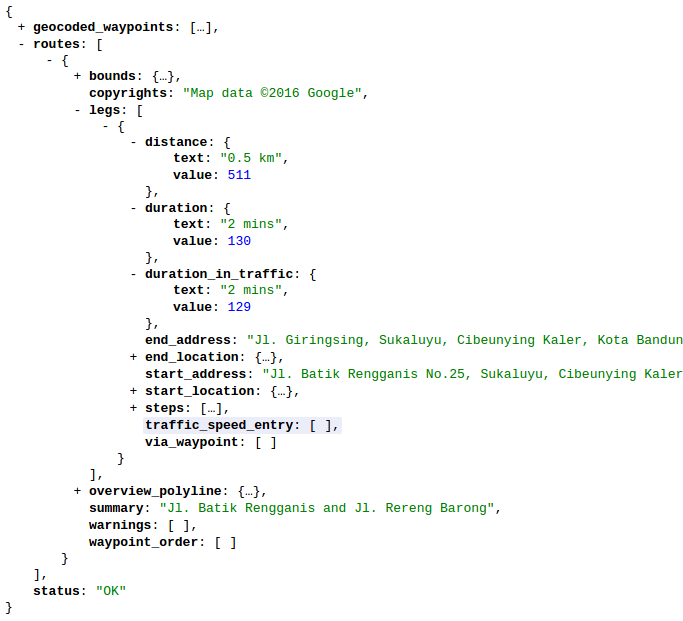
\includegraphics[width=\textwidth]{../../Resources/Images/google_direction_api_response}
	\caption{Google Direction API Response}
	\label{fig:google_direction_api_response}
\end{figure}


Contoh matrix jarak dan waktu tempuh dapat dilihat pada Tabel \ref{tbl:distance_duration_matrix}, sementara data secara lengkap dapat dilihat pada Lampiran \ref{tbl:distance_duration_matrix_full}. Sebagai catatan, jika lokasi \textit{depot} dari pencacah bukan salah satu dari lokasi pencacahan, maka lokasi \textit{depot} juga harus disertakan dalam matriks jarak dan waktu tempuh.


\begin{table}
	\centering
	\ra{1.3}
	\caption{Matriks Jarak dan Waktu Tempuh}
	\label{tbl:distance_duration_matrix}
	\begin{tabular}{llcc}
		\toprule
			Lokasi A & Lokasi B & Jarak & Waktu Tempuh\\
		\midrule
			1302021001 & 1302021003 & 11119 & 1055\\
			1302021001 & 1302021002 & 9373 & 868\\
			1302021001 & 1302021005 & 490 & 38\\
			1302021001 & 1302021004 & 22760 & 2044\\
			...\\
			1302040015 & 1302012010 & 77889 & 8305\\
			1302040014 & 1302100015 & 103893 & 9984\\
			1302040014 & 1302012010 & 73561 & 7546\\
			1302100015 & 1302012010 & 171636 & 16801\\
		\bottomrule
	\end{tabular}
\end{table}


%-----------------------------------------------------------------------------%
\subsection{\textit{Library} dan Implementasi}
%-----------------------------------------------------------------------------%
Terdapat banyak \textit{library} yang dapat digunakan untuk mengatasi permasalahan terkait TSP, mulai dari yang berbayar maupun \textit{open source}. Diantara yang \textit{open source}, terdapat dua library yang cukup lengkap untuk menyelesaikan berbagai variasi dari TSP, yaitu: Jsprit \citep{jsprit_jsprit_2014} dan Optaplanner \citep{optaplanner_constraint_2016}. Pada eksperimen ini digunakan Jsprit, selain dikarenakan lebih mudah dalam implementasi, juga dikarenakan Optaplanner lebih berfokus pada \textit{job scheduling}.

Jsprit merupakan sebuah library berbasis java yang dapat digunakan untuk menyelesaikan permasalahan \textit{traveling salesman problem} (TSP) dan \textit{vehicle routing problems} (VRP). Jsprit mencakup berbagai skenario yang cukup bervariasi, antara lain : \textit{pickups and deliveries}, \textit{back hauls}, \textit{heterogeneous fleets}, \textit{finite and infinite fleets}, \textit{multiple depots}, \textit{time windows}, \textit{open routes}, \textit{different start and end locations}, \textit{multiple capacity dimensions}, \textit{initial loads}, \textit{skills}, dll. Cara kerja Jsprit sangat terstruktur, mulai dari pendefinisan masalah, pemilihan algoritma, pencarian solusi, dan terakhir pemilihan solusi terbaik.


%-----------------------------------------------------------------------------%
\subsubsection{Definisi Masalah}
%-----------------------------------------------------------------------------%
Pendefinisian masalah dengan library Jsprit terdiri dari 3 (tiga) tahapan: definisi lokasi pencacahan, definisi pencacah, dan definisi matriks jarak dan waktu tempuh. Data yang digunakan pada pendefinisian masalah seperti yang telah dijelaskan pada Section \ref{ssec:mtsp_dataset}. Tahap pertama, pendefinisian lokasi pencacahan, dapat dilihat pada Kode \ref{lst:jsprit_define_locations}. Sementara tahap kedua, pendefinisian pencacah, dapat dilihat pada Kode \ref{lst:jsprit_define_enumerators}, dan tahap terakhir, pendefinisan jarak dan waktu tempuh dapat dilihat pada Kode \ref{lst:jsprit_define_route_weights}. Setelah seluruh data dimasukkan, selanjutnya masalah dapat di-\textit{build}, sebagaimana dalam Kode \ref{lst:jsprit_build_problem}.


\begin{listing}
	\caption{Definisi Lokasi Pencacahan}
	\label{lst:jsprit_define_locations}
	\begin{minted}[showspaces=false,breaklines=true]{java}
Service.Builder builder = Service.Builder.newInstance(line[0]);

try {
    Location loc = Location.Builder.newInstance()
        .setId(line[0])
        .setCoordinate(
            Coordinate.newInstance(Double.parseDouble(line[2]), 
                Double.parseDouble(line[1]))).build();
    builder.setLocation(loc);
} catch (Exception e) {}

Service node = builder.build();
vrpBuilder.addJob(node);
	\end{minted}
\end{listing}


\begin{listing}
	\caption{Definisi Pencacah dari File .csv}
	\label{lst:jsprit_define_enumerators}
	\begin{minted}[showspaces=false,breaklines=true]{java}
VehicleTypeImpl.Builder vehicleTypeBuilder = VehicleTypeImpl.Builder.newInstance("enumerator");
vehicleTypeBuilder.setCostPerDistance(0);
vehicleTypeBuilder.setCostPerTransportTime(1);
vehicleTypeBuilder.setCostPerServiceTime(1);
VehicleType vehicleType = vehicleTypeBuilder.build();

VehicleImpl.Builder builder = VehicleImpl.Builder.newInstance(line[0]);

try {
    Location loc = Location.Builder.newInstance()
            .setId(line[0])
            .setCoordinate(Coordinate.newInstance(Double.parseDouble(line[2]),
                    Double.parseDouble(line[1])))
            .build();
    builder.setStartLocation(loc);
} catch (Exception e) {}


builder.setType(vehicleType);
VehicleImpl vehicle = builder.build();
vrpBuilder.addVehicle(vehicle);
	\end{minted}
\end{listing}


\begin{listing}
	\caption{Definisi Penimbang Jarak dan Waktu Tempuh dari File .csv}
	\label{lst:jsprit_define_route_weights}
	\begin{minted}[showspaces=false,breaklines=true]{java}
VehicleRoutingTransportCostsMatrix.Builder costMatrixBuilder = VehicleRoutingTransportCostsMatrix.Builder
        .newInstance(true);

while ((line = reader.readNext()) != null) {
    try {
        costMatrixBuilder.addTransportDistance(line[0], line[1], Double.parseDouble(line[2]));
        costMatrixBuilder.addTransportTime(line[0], line[1], Double.parseDouble(line[3]));
    } catch (Exception e) {
        costMatrixBuilder.addTransportDistance(line[0], line[1], 0.0);
        costMatrixBuilder.addTransportTime(line[0], line[1], 0.0);
    }
}

VehicleRoutingTransportCosts costMatrix = costMatrixBuilder.build();
vrpBuilder.setRoutingCost(costMatrix);
	\end{minted}
\end{listing}


\begin{listing}
	\caption{Build Problem}
	\label{lst:jsprit_build_problem}
	\begin{minted}[showspaces=false,breaklines=true]{java}
VehicleRoutingProblem.Builder vrpBuilder = VehicleRoutingProblem.Builder.newInstance();
vrpBuilder.setFleetSize(VehicleRoutingProblem.FleetSize.FINITE);
VehicleRoutingProblem problem = vrpBuilder.build();
	\end{minted}
\end{listing}


%-----------------------------------------------------------------------------%
\subsubsection{Definisi Algoritma}
%-----------------------------------------------------------------------------%
Setelah masalah di-\textit{build}, selanjutnya Jsprit akan membuat algoritma dari masalah yang telah didefinisikan sebelumnya secara \textit{out-of-the-box}. Pada tahap ini juga dapat ditentukan berapa jumlah iterasi yang akan digunakan, dan thread yang akan digunakan dalam pencarian solusi. Kode \ref{lst:jsprit_create_algorithm} menunjukkan bagaimana Jsprit menciptakan algoritma.


\begin{listing}
	\caption{Penentuan Algoritma}
	\label{lst:jsprit_create_algorithm}
	\begin{minted}[showspaces=false,breaklines=true]{java}
VehicleRoutingAlgorithm algorithm = Jsprit.Builder.newInstance(problem)
        .setProperty(Jsprit.Parameter.THREADS, 5).buildAlgorithm();
algorithm.setMaxIterations(iterations);
	\end{minted}
\end{listing}


%-----------------------------------------------------------------------------%
\subsubsection{Pencarian Solusi dan Penentuan Solusi Terbaik}
%-----------------------------------------------------------------------------%
Setelah algoritma dibuat, selanjutnya proses pencarian solusi dapat dilakukan. Pada tahapan ini, akan ditemukan lebih dari satu solusi terbaik, sehingga perlu dipilih solusi terbaik dari sejumlah solusi tersebut. Kode \ref{lst:jsprit_search_solution} menunjukkan bagaimana pencarian solusi oleh Jsprit dilakukan.


\begin{listing}
	\caption{Pencarian Solusi}
	\label{lst:jsprit_search_solution}
	\begin{minted}[showspaces=false,breaklines=true]{java}
Collection<VehicleRoutingProblemSolution> solutions = algorithm.searchSolutions();
VehicleRoutingProblemSolution bestSolution = Solutions.bestOf(solutions);
	\end{minted}
\end{listing}


%-----------------------------------------------------------------------------%
\subsection{Hasil dan Analisis}
%-----------------------------------------------------------------------------%
Dari eksperimen diatas, diperoleh rekomendasi seperti Gambar \ref{fig:analysis_mtsp_recommendation}, atau Listing \ref{lst:analysis_mtsp_recommendation} untuk detail dari masing-masing pencacah. Jika \textit{service time} diketahui mengikuti distribusi \textit{normal}, seperti pada Lampiran \ref{tbl:location_service_times}, maka dapat diperoleh rata-rata dan standar deviasi waktu penyelesaian untuk masing-masing pencacah adalah:
$$ \mu = 82.24 jam $$
$$ \sigma = 88.95 jam $$


\begin{figure}[h]
	\centering
	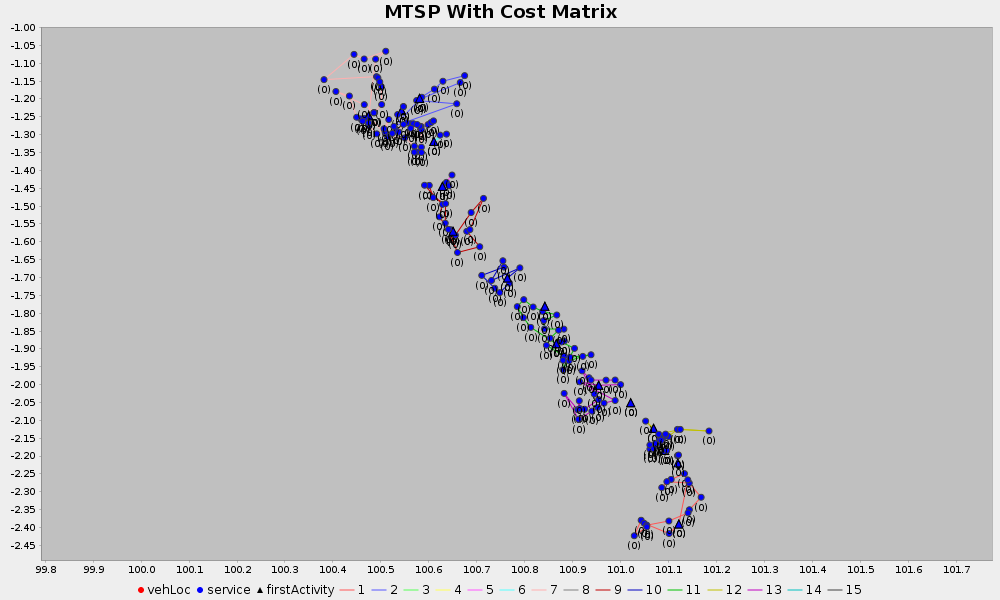
\includegraphics[width=\textwidth]{../../Resources/Images/analysis_mtsp_no_time_windows}
	\caption{Grafik Rekomendasi dengan MTSP}
	\label{fig:analysis_mtsp_recommendation}
\end{figure}


\begin{listing}[h]
	\caption{Rekomendasi dengan MTSP}
	\label{lst:analysis_mtsp_recommendation}
	\begin{minted}[showspaces=false,breaklines=true, escapeinside=||]{text}
|\textbf{1302021005}| : 1302021001 --> 1302021005
|\textbf{1302101005}| : 1302101005 --> 1302101001 --> 1302100010 --> 1302100014 --> 1302100011 --> 1302101004 --> 1302101006 --> 1302101003 --> 1302101002
|\textbf{1302070006}| : 1302070006 --> 1302070002 --> 1302070003 --> 1302080009 --> 1302080004 --> 1302080001 --> 1302080005 --> 1302080003 --> 1302070012 --> 1302070011 --> 1302070001 --> 1302070004 --> 1302070007 --> 1302070008 --> 1302070010 --> 1302070009 --> 1302070005
|\textbf{1302050007}| : 1302050007
|\textbf{1302100002}| : 1302100002 --> 1302100003 --> 1302100013 --> 1302100012
|\textbf{1302030005}| : 1302030005
|\textbf{1302110003}| : 1302110003 --> 1302100001 --> 1302090006 --> 1302090012 --> 1302090003 --> 1302090014 --> 1302090009 --> 1302090015 --> 1302090018 --> 1302090016 --> 1302090017 --> 1302090013 --> 1302090005 --> 1302090007 --> 1302090002 --> 1302090008 --> 1302090001 --> 1302100015 --> 1302100004 --> 1302100016 --> 1302090011 --> 1302090010 --> 1302100017 --> 1302100006 --> 1302100007 --> 1302100009 --> 1302100008 --> 1302100005 --> 1302110001 --> 1302110010 --> 1302110013 --> 1302110002 --> 1302110014 --> 1302110015 --> 1302110011 --> 1302110016 --> 1302110017 --> 1302110004 --> 1302110018 --> 1302110019 --> 1302110005 --> 1302110012 --> 1302110023 --> 1302110020 --> 1302110006 --> 1302110007 --> 1302110008 --> 1302110021 --> 1302110009 --> 1302110022
|\textbf{1302012003}| : 1302012007 --> 1302012003 --> 1302012008
|\textbf{1302080006}| : 1302080006 --> 1302080008 --> 1302080002 --> 1302080007
|\textbf{1302031005}| : 1302031005 --> 1302031008 --> 1302030014 --> 1302030006 --> 1302030009 --> 1302030004 --> 1302030010 --> 1302031003 --> 1302030002 --> 1302031004 --> 1302030003 --> 1302030012 --> 1302031001 --> 1302031006 --> 1302040011 --> 1302031009 --> 1302031010 --> 1302031002 --> 1302031007 --> 1302030001
|\textbf{1302060005}| : 1302060005 --> 1302060009 --> 1302060006 --> 1302060008 --> 1302060002 --> 1302060007 --> 1302060001 --> 1302060003 --> 1302060004
|\textbf{1302020006}| : 1302020006 --> 1302020015 --> 1302020011 --> 1302020009 --> 1302020010 --> 1302020001 --> 1302020003 --> 1302020005 --> 1302021006 --> 1302021002 --> 1302021007 --> 1302021008 --> 1302021003 --> 1302021009 --> 1302021004 --> 1302021010 --> 1302020016 --> 1302020017
|\textbf{1302011008}| : 1302011008 --> 1302011007 --> 1302011004 --> 1302011003 --> 1302011002 --> 1302011006 --> 1302011005 --> 1302011009 --> 1302011010 --> 1302011001 --> 1302012005 --> 1302012002 --> 1302012009 --> 1302012010 --> 1302012004 --> 1302012001 --> 1302012006
|\textbf{1302040002}| : 1302040002 --> 1302040003 --> 1302040004 --> 1302040015 --> 1302040008 --> 1302040009 --> 1302040010 --> 1302040014 --> 1302040012 --> 1302040013 --> 1302040001 --> 1302040016 --> 1302040007 --> 1302040006 --> 1302040005 --> 1302050001 --> 1302050004 --> 1302050006 --> 1302050002 --> 1302050008 --> 1302050010 --> 1302050009 --> 1302050005 --> 1302050003
|\textbf{1302090004}| : 1302090004 --> 1302090019 --> 1302090020
	\end{minted}
\end{listing}


\begin{table}
	\centering
	\ra{1.3}
	\caption{Total Waktu Setiap Pencacah dengan MTSP}
	\label{tbl:enumerators_total_time}
	\begin{tabular}{lc}
		\toprule
			Pencacah & Total Waktu (jam)\\
		\midrule
			1302021005 & 13.3\\
			1302101005 & 60.8\\
			1302070006 & 116\\
			1302050007 & 6\\
			1302100002 & 26.6\\
			1302030005 & 6\\
			1302110003 & 341\\
			1302012003 & 19.9\\
			1302080006 & 27.1\\
			1302031005 & 136\\
			1302060005 & 61.3\\
			1302020006 & 121\\
			1302011008 & 116\\
			1302040002 & 162\\
			1302090004 & 20.2\\
		\bottomrule
	\end{tabular}
\end{table}


Dari eksperimen, dapat diketahui metode MTSP tidak cocok digunakan untuk menentukan rekomendasi yang sensitif terhadap \textit{time windows}, namun datanya tidak tersedia sampai dengan lokasi dikunjungi. Untuk itu MTSP perlu dikombinasikan dengan metode lain, sehingga dapat memberikan rekomendasi dengan lebih akurat.


Solusi yang ditawarkan untuk menyelesaikan kasus rekomendasi lokasi pencacahan adalah dengan menggunakan \textit{real-time} MTSP. Ada berbagai cara untuk mengimplementasikan \textit{real-time system}, yang paling umum adalah dengan menggunakan \textit{Web service}. \textit{Web service} bekerja secara \textit{synchronous}, dimana setiap \textit{request} dan \textit{reply} akan diproses secara berurutan. Arsitektur semacam ini tidak cocok digunakan dalam aplikasi yang bersifat \textit{information driven} \citep{muhl_large-scale_2002}. Sebagai alternatif, paradigma \textit{publish/subscribe} dapat digunakan, karena paradigma \textit{publish/subscribe} memungkinkan \textit{client/subscriber} dan \textit{server/publisher} berkomunikasi secara tidak langsung.


%-----------------------------------------------------------------------------%
\section{Perancangan}
\label{sec:design}
%-----------------------------------------------------------------------------%


%-----------------------------------------------------------------------------%
\subsection{\textit{System Overview}}
%-----------------------------------------------------------------------------%
Sebagaimana disampaikan sebelumnya, kekurangan algoritma MDVRP ketika digunakan begitu saja dalam rekomendasi lokasi untuk pengumpulan data lapangan adalah ketiadaan data waktu kunjungan (\textit{time service}), yang mana memiliki peranan penting dalam kalkulasi rekomendasi. Untuk itu algoritma MDVRP perlu diintegrasikan dengan suatu mekanisme \textit{real-time}. Terdapat beberapa mekanisme yang bisa diadopsi untuk sistem \textit{real-time}, antara lain: Web Service, Remote Procedure Call (RPC), message passing, dan publish/service \citep{eugster_many_2003}.


Pada penelitian ini digunakan mekanisme \textit{publish/subscribe}, karena \textit{publish/subscribe} memiliki karakteristik \textit{loose coupling}. Terlebih lagi mekanisme \textit{publish/subscribe} juga cocok digunakan pada sistem yang bersifat \textit{information-driven} \citep{muhl_large-scale_2002}. Karena karakteristiknya ini, \textit{publish/subscribe} dapat bekerja secara \textit{synchronous}, dimana \textit{request} dan \textit{reply} tidak harus diproses secara berurutan. \textit{Publisher} dapat melakukan \textit{publish} dalam kondisi \textit{offline}, begitu juga \textit{subscriber} dapat melakukan \textit{subscribe} ketika offline.


\begin{figure}[h]
	\centering
	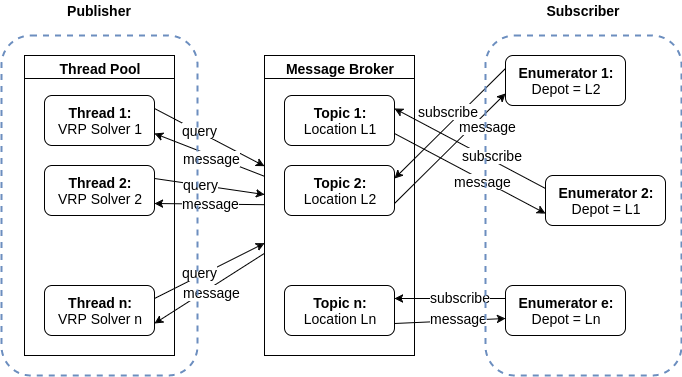
\includegraphics[width=\textwidth]{../../Resources/Images/system-overview}
	\caption{Garis Besar Sistem}
	\label{fig:system-overview}
\end{figure}


Gambar \ref{fig:system-overview} menunjukkan garis besar sistem yang terdiri dari 3 (tiga) komponen utama, yaitu: \textit{publisher}, \textit{subscriber}, dan \textit{message broker}. Komunikasi yang terjadi antara \textit{publisher} dan \textit{subscriber} disusun atas dasar kesamaan \textit{event} atau \textit{topic}. Pada penelitian ini, topi yang digunakan sebagai dasar komunikasi antara \textit{publisher} dan \textit{subscriber} adalah \textit{current location} dari masing-masing \textit{subscriber}.


Paradigma \textit{publish/subscribe} secara umum tersusun dari 3 (tiga) komponen: \textit{subscriber}, \textit{message broker}, dan \textit{publisher} \citep{banavar_efficient_1999}. \textit{Subscriber} dalam konteks sistem rekomendasi lokasi pencacahan adalah setiap pencacah yang menginginkan informasi tentang suatu topik. Topik dalam konteks ini adalah "lokasi pencacahan saat ini" dari setiap pencacah. Pemilihan "lokasi pencacahan saat ini" sebagai topik karena "lokasi pencacahan saat ini" bersifat \textit{unique}, dimana satu lokasi pencacahan hanya dikunjungi oleh satu pencacah, sehingga sebuah topik hanya akan mempunyai satu \textit{subscriber}.


Sementara \textit{publisher} adalah satu atau lebih sistem yang mem-\textit{publish} informasi tentang lokasi pencacahan selanjutnya dari setiap topik. Dan \textit{message broker} bertanggung jawab mengakomodir seluruh topik yang di-\textit{subscribe}, dan menyebarluaskan setiap informasi yang di-\textit{publish} kepada client yang men-\textit{subscribe}-nya. Gambar \ref{fig:system-overview} menggambarkan garis besar sistem rekomendasi lokasi berbasis \textit{publish/subscribe}.


%-----------------------------------------------------------------------------%
\subsection{\textit{TSP Solver}}
%-----------------------------------------------------------------------------%
Terdapat beberapa algoritma yang dapat digunakan untuk menyelesaikan permasalahan TSP, atau lebih spesifik MDVRP, seperti: tabu search (CGL) \citep{cordeau_tabu_1997}, adaptive large neighborhood search (ALNS) \citep{pisinger_general_2007}, fuzzy logic guided genetic algorithm (FLGA) \citep{lau_application_2010}, paralel iterated tabu search (ITS) \citep{cordeau_parallel_2012}, hybrid algorithm combining Iterated Local Search and Set Partitioning (ILS-RVND-SP) \citep{subramanian_hybrid_2013}, hybrid genetic algorithm with adaptive diversity control (HGSADC+) \citep{vidal_implicit_2014}, hybrid Granular Tabu Search (ELTG) \citep{escobar_hybrid_2014}, dan cooperative coevolutionary strategies (CoES) \citep{de_oliveira_cooperative_2016}. Dalam kasus ini akan digunakan algoritma CoES, karena CoES menghasilkan \textit{mean solution values} yang competitive dengan \textit{CPU time} yang relatif lebih rendah.


Pada \textit{cooperative coevolutionary algorithm}, \citep{engelbrecht_coevolution_2007}, masalah dapat dipecah menjadi beberapa masalah yang lebih kecil (\textit{sub-problem}). Setiap populasi berkembang pada masing-masing \textit{sub-problem}. Setelah melalui sejumlah generasi, individu pada populasi-populasi tersebut bergabung membentuk solusi yang lengkap. Melalui proses ini, maka dimungkinkan untuk menghitung \textit{fitness} dari solusi lengkap. Sejumlah informasi kemudian dikembalikan kepada setiap populasi, seperti solusi terbaik yang ditemukan sejauh ini, dan \textit{update} untuk individu dalam populasi. Gambar \ref{fig:coes_overview} memberikan gambaran umum tentang cara kerja dari \textit{cooperative coevolutionary algorithm} \citep{de_oliveira_cooperative_2016}.


\begin{figure}[h]
	\centering
	
\includegraphics[width=10cm]{../../Resources/Images/coes_overview}
	\caption{\textit{Cooperative coevolutionary} algorithm dengan \textit{problem decomposition}}
	\label{fig:coes_overview}
\end{figure} 


%-----------------------------------------------------------------------------%
\subsubsection{\textit{Cooperative Coevolutionary Model} pada \textit{MDVRP}}
%-----------------------------------------------------------------------------%
Langkah pertama pada \textit{cooperative coevolutionary algorithm} adalah dekomposisi \textit{problem} menjadi \textit{sub-problem}. Setiap \textit{sub-problem} akan menjadi \textit{single-depot} VRP. Pada proses dekomposisi ini memungkinkan terjadinya \textit{overlap}, dimana \textit{customer} dapat diasosiasikan terhadap satu atau lebih \textit{depot}, tergantung dari lingkungannya. \textit{Customer} diasosiasikan pada \textit{depot} dengan mengikuti 2 (dua) aturan:
\begin{inparaenum}[1)]
\item \textit{Depot} terdekat,
\item \textit{Depot} dari node terdekat
\end{inparaenum}.
Jika kedua aturan tersebut menghasilkan \textit{depot} yang berbeda, maka konflik harus diselesaikan dengan cara tertentu. Gambar \ref{fig:coes_problem_decomposition} mengilustrasikan bagaimana kedua rule tersebut diimplementasikan.


\begin{figure}[h]
	\centering
	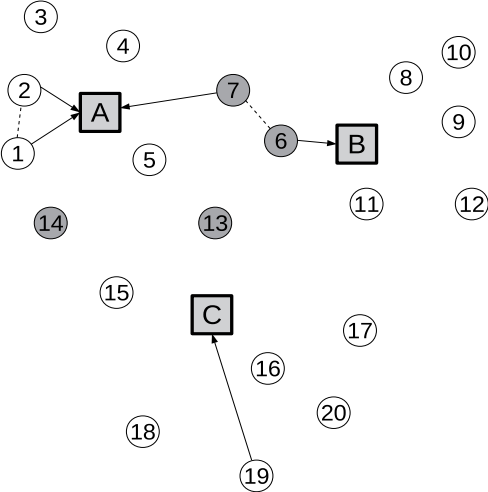
\includegraphics[width=7cm]{../../Resources/Images/coes_problem_decomposition}
	\caption{\textit{Problem decomposition}: alokasi \textit{customer} ke \textit{depot}}
	\label{fig:coes_problem_decomposition}
\end{figure}


%-----------------------------------------------------------------------------%
\subsubsection{\textit{Paralel Evolution Strategy}}
%-----------------------------------------------------------------------------%
Setelah \textit{problem} didekomposisi menjadi \textit{sub-problem}, kemudian populasi untuk setiap \textit{sub-problem} diinisiasi dengan menggunakan metode \textit{Nearest Insertion Heuristic (NIH)} \citep{raff_routing_1983}. Pada NIH, \textit{customer} yang paling dekat dengan setiap \textit{depot} dimasukkan dalam rute, kemudian \textit{customer} kedua yang paling dekat dengan \textit{customer} pertama dimasukkan, dan seterusnya sampai seluruh \textit{customer} dimasukkan.


Langkah selanjutnya adalah dengan menjalankan \textit{paralel module and coordination} sampai dengan \textit{stop condition} tercapai. Terdapat 3 (tiga) \textit{module} yang harus dijalankan, yaitu: \textit{Population Evolve} (PE), \textit{Complete Solution Evaluation} (CSE), dan \textit{Elite Group} (EG). Gambar \ref{fig:coes_paralel_modules} menggambarkan arsitektur pada \textit{paralel module}.


\begin{figure}[h]
	\centering
	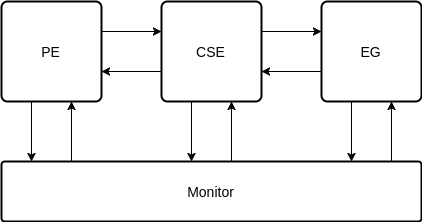
\includegraphics[width=7cm]{../../Resources/Images/coes_paralel_modules}
	\caption{Arsitektur \textit{paralel module} di CoES}
	\label{fig:coes_paralel_modules}
\end{figure}


Masing-masing \textit{module}, PE, CSE, dan EG dijalankan dalam \textit{thread} terpisah. Sementara \textit{Monitor module} memanage proses paralel pada \textit{module} dan mengirimkan informasi mengenai \textit{problem} yang akan diselesaikan. Ketika \textit{stop condition} tercapai, \textit{Monitor module} menghentikan semua \textit{module} dan solusi yang diperoleh menjadi solusi terbaik.


\textit{Population Evolve} module adalah module yang memanage evolusi dari setiap populasi berdasarkan \textit{ES (evolution strategies)}. Gambar \ref{fig:coes_pe_module} menggabarkan arsitektur dari \textit{PE module}.


\begin{figure}[h]
	\centering
	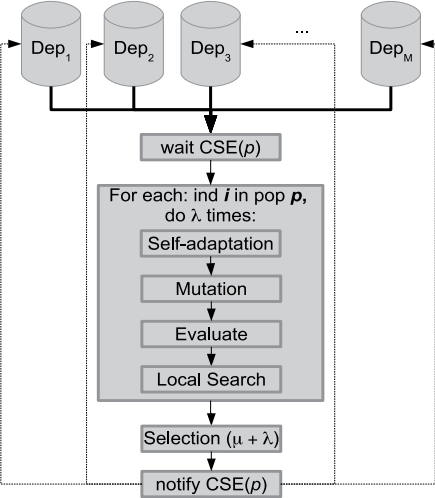
\includegraphics[width=7.5cm]{../../Resources/Images/coes_pe_module}
	\caption{Arsitektur \textit{Population Evolve module} di CoES}
	\label{fig:coes_pe_module}
\end{figure}


\textit{Complete Solutions Evaluate module} mengambil populasi dari \textit{partial solution} dari seluruh \textit{PE module}, menggabungkannya menjadi solusi lengkap, kemudian mengevaluasi \textit{global fitness} dari solusi lengkap tersebut. Pada prosesnya, masing-masing individu dari sebuah populasi digabungkan dengan individu terbaik dari populasi yang lain untuk membentuk solusi lengkap. Individu terbaik diperoleh dari \textit{Elite Group module}.


Solusi lengkap yang terbentuk masih memungkinkan adanya duplikasi \textit{customer} maupun \textit{missing customer}, untuk itu diperlukan adanya \textit{repair procedure}. Pada \textit{repair procedure} digunakan \textit{least additional cost heuristics} \citep{raff_routing_1983}, baik untuk menghilangkan duplikasi \textit{customer} maupun menambahkan \textit{missing customer}. Ilustrasi dari \textit{CSE module} dapat dilihat pada Gambar \ref{fig:coes_cse_module}.


\begin{figure}[h]
	\centering
	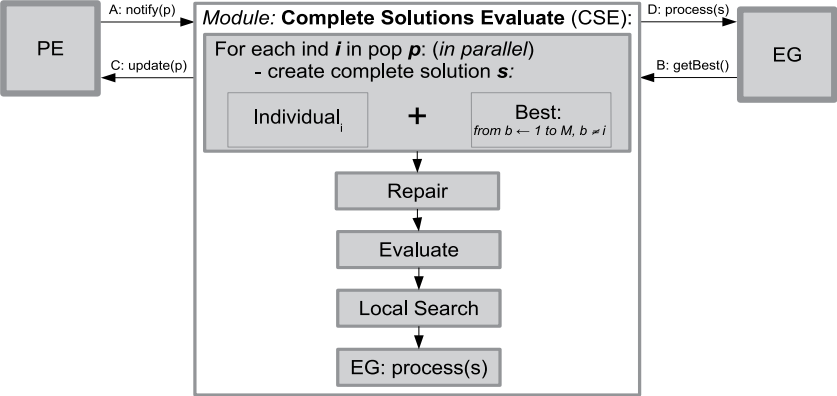
\includegraphics[width=\textwidth]{../../Resources/Images/coes_cse_module}
	\caption{Arsitektur \textit{Complete Solution Evaluation module} di CoES}
	\label{fig:coes_cse_module}
\end{figure}


Sementara itu \textit{Elite Group module} mengelola sebuah set berisi $\tau$ dari solusi lengkap, termasuk didalamnya solusi lengkap \textit{global}, yang dikirimkan oleh modul CSE. Jika set berisi kurang dari $\tau$ solusi lengkap, maka solusi yang baru dapat secara langsung dimasukkan ke dalam set. Sebaliknya, jika set telah berisi sejumlah $\tau$ solusi lengkap, maka solusi yang baru hanya dapat dimasukkan jika lebih baik dari solusi terburuk yang ada didalam set. Ilustrasi dari \textit{EG module} dapat dilihat pada Gambar \ref{fig:coes_eg_module}.


\begin{figure}[h]
	\centering
	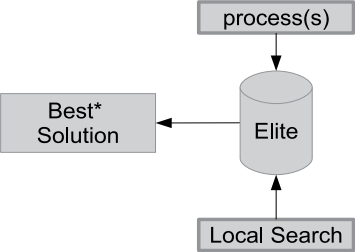
\includegraphics[width=5cm]{../../Resources/Images/coes_eg_module}
	\caption{Arsitektur \textit{Elite Group module} di CoES}
	\label{fig:coes_eg_module}
\end{figure}


%-----------------------------------------------------------------------------%
\subsection{\textit{Publisher}}
%-----------------------------------------------------------------------------%


Setiap \textit{publisher} dalam sistem mengimplementasikan \textit{Travelling Salesman Problem (TSP) solver}. Setiap \textit{problem} yang diproses oleh setiap \textit{instance} dari \textit{TSP solver} mengikutsertakan seluruh pencacah (dinotasikan dengan $M$) sebagai \textit{salesman} dan seluruh blok sensus yang belum di\textit{assign} sebagai \textit{customer} (dinotasikan dengan $N$). Hal ini dikarenakan \textit{TSP solver} menggunakan \textit{total route costs} sebagai \textit{fitness value}, sehingga berpotensi terjadi \textit{local best solution}. Maksud dari \textit{local best solution} adalah solusi yang dihasilkan adalah solusi terbaik bagi seorang pencacah saja, yang sebenarnya akan lebih baik jika \textit{lokasi} pada solusi tersebut di\textit{assign} kepada pencacah lain.


Setiap \textit{subscribe} akan diproses dalam satu \textit{session}. Solusi terbaik yang diperoleh akan berisi minimum satu rute, dan maksimum berisi $M$ rute. Jika pada solusi terbaik yang dihasilkan oleh sebuah \textit{session} tidak terdapat alokasi rute untuk \textit{subscriber} dari \textit{session} tersebut, maka \textit{session} tersebut akan diproses ulang tanpa melibatkan pencacah yang lain. Mekanisme ini dimaksudkan untuk memastikan setiap \textit{session subscriber} mendapatkan alokasi rute. Prosedur yang diusulkan pada publisher seperti pada Algoritma \ref{lst:proposed_solver_thread_algorithm} dan Algoritma \ref{lst:proposed_publisher_algorithm}.


\begin{listing}
	\caption{Algoritma TSPSolver Thread}
	\label{lst:proposed_solver_thread_algorithm}
	\begin{minted}[showspaces=false,breaklines=true,escapeinside=||]{python}
createSolverThread(|$C_{i}$|, |$E_{1}$|...|$E_{M}$|, |$L_{1}$|...|$L_{unsolved(N)}$|)
	|$S_{C_{i}}$| <- TspSolver(|$C_{i}$|, |$E_{1}$|...|$E_{M}$|, |$L_{1}$|...|$L_{unsolved(N)}$|)
	for |$c$| <- 1 to |$len(S_{C_{i}})$| do
		rec <- publish(|$S_{c}$|, |$S_{R_{1}}$|);
		if rec > 0 do
			cancelThread(|$S_{c}$|)
		end if
	end for
	if |$C_{i}$| not in |$S_{C_{i}}$| do
		createSolverThread(|$E_{C_{i}}$|, |$E_{1}$|...|$E_{M}$|, |$L_{1}$|...|$L_{unsolved(N)}$|)
	end if
	cancelThread(|$T_{i}$|)
end
	\end{minted}
\end{listing}


\begin{listing}
	\caption{Algoritma Publisher}
	\label{lst:proposed_publisher_algorithm}
	\begin{minted}[showspaces=false,breaklines=true,escapeinside=||]{python}
|$C$| <- readChannels()
for |$i$| <- 1 to |$len(C)$| do
	if |$C_{i}$| not in |$T$| do
		|$T_{i}$| <- createSolverThread(|$C_{i}$|, |$E_{1}$|...|$E_{M}$|, |$L_{1}$|...|$L_{unsolved(N)}$|);
	end if
end for
	\end{minted}
\end{listing}


Arsitektur \textit{publish/subscribe} merupakan sebuah arsitektur yang bersifat \textit{loose coopling}, dimana antara \textit{publisher} dan \textit{subscriber} tidak saling mengetahui \citep{muhl_large-scale_2002}. Salah satu konsekuensinya, ketika seorang pencacah melakukan \textit{subscribe}, pada saat solusi diperoleh pencacah tersebut sudah terputus dari \textit{broker}. Untuk itu diperlukan mekanisme \textit{caching}, sehingga pada saat pencacah terkoneksi kembali dengan \textit{broker}, maka solusi yang terdapat pada \textit{cache} dapat langsung di\textit{pusblish}.


%-----------------------------------------------------------------------------%
\subsection{\textit{Message Broker}}
%-----------------------------------------------------------------------------%
\textit{Message broker} adalah sebuah komponen yang bertanggung jawab dalam menyalurkan (\textit{routing}) pesan dari \textit{publisher} ke \textit{subscriber} sesuai dengan topik yang di\textit{subscribe} \citep{banavar_efficient_1999}. Suatu sistem \textit{publish/subscribe} dapat memiliki \textit{single broker} maupun \textit{multi broker}. Pada arsitektur \textit{single broker}, seluruh \textit{subscriber} dan \textit{publisher} terkoneksi pada satu \textit{broker}, sementara pada \textit{multi broker}, setiap \textit{subscriber} maupun \textit{publisher} dapat terkoneksi pada broker terdekat. Arsitektur \textit{multi depot} ini juga disebut dengan \textit{distributed pub/sub system} \citep{muhl_large-scale_2002}, seperti ilustrasi pada Gambar \ref{fig:pub_sub_distributed_ilustration}. Adapun rancangan yang diusulkan akan menerapkan arsitektur terdistribusi, dikarenakan lokasi pencacahan secara geografis tersebar.


\begin{figure}[h]
	\centering
	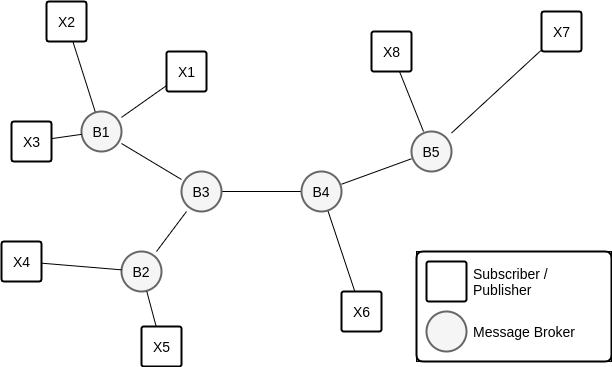
\includegraphics[width=9cm]{../../Resources/Images/pub_sub_distributed_ilustration}
	\caption{Arsitektur \textit{Publish-Subscribe} terdistribusi}
	\label{fig:pub_sub_distributed_ilustration}
\end{figure}


%#############################################################################%
\begin{comment}
%-----------------------------------------------------------------------------%
\subsection{\textit{Search Algorithm}}
%-----------------------------------------------------------------------------%
Terdapat berbagai variasi algoritma untuk menyelesaikan permasalah TSP maupun VRP, antara lain: genetic algorithm, simmulated annealing, tabu search, particle swarm optimization, harmony search, quantum annealing, greedy 2-opt, dll. Pada pengujian yang dilakukan dengan kasus single-salesman dengan menggunakan 3 (tiga) kriteria: \textit{mean quality}, \textit{dispersion of quality}, dan \textit{time needed to reach the optimum}, simmulated annealing menghasilkan solusi yang paling berkualitas, sementara tabu search merupakan yang paling baik dari sisi performance \citep{antosiewicz_choice_2013}.


%-----------------------------------------------------------------------------%
\subsection{\textit{Greedy Strategy}}
%-----------------------------------------------------------------------------%
Algoritma \textit{greedy} adalah suatu algoritma yang menentukan solusi optimal berdasarkan kondisi saat ini, atau disebut dengan \textit{local optimum}. Algoritma greedy dapat meminimalisir waktu komputasi dalam pencarian solusi global. Pada kasus \textit{travelling salesman problem}, strategi greedy dapat dikatakan dengan "pada setiap tahap, kunjungi kota yang paling dekat dengan lokasi salesman yang belum dikunjungi" \citep{paul_e._black_greedy_2005}. 


Pada metode MTSP, diperoleh lebih dari satu solusi, dimana masing-masing solusi diperbandingkan. Perbandingan dilakukan berdasarkan \textit{cost} keseluruhan, dimana solusi dengan \textit{cost} terkecil adalah solusi terbaik.


Penentuan solusi terbaik dengan membandingkan \textit{cost} keseluruhan tidaklah tepat. \textit{Cost} ditentukan dengan satuan waktu, sementara salah satu komponen utama yang dominan adalah \textit{service time}. Karena \textit{service time} tidak tersedia, maka membandingkan keseluruhan waktu akan menjadi bias. Hipotesis yang ditawarkan adalah membandingkan setiap solusi dengan total \textit{cost} untuk lokasi pertama dari masing-masing pencacah saja, karena lokasi pertama tidak terpengaruh dengan \textit{service time}, seperti algoritma dalam Kode \ref{lst:proposed_best_solution_algorithm}.


\begin{listing}
	\caption{Algoritma Solusi Terbaik}
	\label{lst:proposed_best_solution_algorithm}
	\begin{minted}[showspaces=false,breaklines=true]{python}
Let E be all enumerators
Let L be all locations
Run MTSP with enumerators E and locations L
Let S be all solutions from MTSP
Let Cs be an empty dict
For each solution s in S do
	Let R be all routes in solution s
	Let C be 0
	For each route r in R do
		Let J be all jobs in route r
		Let fj be first job in J
		Let cfj be cost of first job fj
		Add C with cjf
	Put C in dict Cs with key solution s
	
Let element in dict Cs with the least value be the best solution
	\end{minted}
\end{listing}


Algoritma \ref{lst:proposed_best_solution_algorithm} merupakan rekomendasi lokasi pertama untuk setiap pencacah. Selanjutnya pencacah dapat melakukan pengumpulan data pada lokasi tersebut sampai selesai, dengan \textit{service time} bervariasi, sehingga waktu selesai pencacahan berbeda-beda antar pencacah. Setiap pencacah yang telah menyelesaikan pengumpulan data, dapat melakukan \textit{subscribe} solusi yang baru kepada \textit{broker}, seperti algoritma pada Kode \ref{lst:proposed_subscribe_solution_algorithm}. Setiap kali broker mendapati adanya \textit{subscribers}, maka \textit{broker} akan mencari solusi baru dengan metode MTSP. Solusi yang dicari hanya menyertakan \textit{subscribers} saja, dan meng-\textit{exclude} lokasi yang telah dikunjungi, seperti algoritma pada Kode \ref{lst:proposed_subscribers_best_solution_algorithm}.


\begin{listing}
	\caption{Algoritma \textit{Subscribe Solution}}
	\label{lst:proposed_subscribe_solution_algorithm}
	\begin{minted}[showspaces=false,breaklines=true]{python}
Let SS be an empty list
For each e in enumerators E do
	If enumerator e has finished enumerating do
		Exclude location l enumerated by e from locations L
		Add e in list of subscribers SS
	\end{minted}
\end{listing}


\begin{listing}
	\caption{Algoritma Solusi Terbaik untuk \textit{Subscribers}}
	\label{lst:proposed_subscribers_best_solution_algorithm}
	\begin{minted}[showspaces=false,breaklines=true]{python}
While locations L is not empty do
	Run MTSP with enumerators SS and locations L
    Let S be all solutions from MTSP
    Let Cs be an empty dict
    For each solution s in S do
	    Let R be all routes in solution s
	    Let C be 0
	    For each route r in R do
		    Let J be all jobs in route r
		    Let fj be first job in J
		    Let cfj be cost of first job fj
		    Add C with cjf
	    Put C in dict Cs with key solution s
	
    Let Bs as element in dict Cs with the least value
    Publish Bs to all subscribers SS
    Set subscribers SS to empty list
	\end{minted}
\end{listing}


%-----------------------------------------------------------------------------%
\subsection{\textit{Publish/Subscribe Paradigm}}
%-----------------------------------------------------------------------------%








\section{Garis Besar Perancangan}

Alur kerja perancangan dimulai dengan dengan mengidentifikasi blok sensus yang akan dilakukan pendataan padanya, serta menentukan jumlah pencacah yang akan digunakan. Kedua permasalahan ini tidak akan dibahas terlalu mendalam dalam penelitian ini. Lokasi pencacahan telah ditentukan dalam fase perancangan sensus dan survei, mengikuti sebuah metodologi tertentu. Sementara jumlah pencacahan juga telah ditentukan, mengikuti jumlah sampel dan berbagai persyaratan tertentu, seperti waktu dan biaya.


Selanjutnya, setiap pencacah akan dialokasikan kepada blok sensus yang akan dicacah dengan menggunakan metode MTSP, sebagaimana diformulasikan oleh \citep{bektas_multiple_2006}, dengan ketentuan setiap pencacah dapat memulai dan mengakhiri pada \textit{depot} yang berbeda-beda. Setelah model diperoleh, setiap pencacah akan mengunjungi lokasi pertama dari rekomendasi. Setelah selesai kunjungan, lokasi akan disimpan dalam \textit{tabu list} dengan menggunakan metode pub-sub \citep{chen_efficient_2003}. Model baru akan digenerate setiap kali terdapat \textit{request} dari salah satu pencacah. Setiap kali model di-\textit{generate}, \textit{tabu search} \citep{glover_tabu_1989, glover_tabu_1990} yang memanfaatkan \textit{tabu list} akan digunakan untuk memastikan tidak terdapat \textit{conflict}. Setelah model baru selesai di-\textit{generate}, maka mudel akan di-\textit{publish} kepada setiap pencacah yang telah men-\textit{subscribe}.


\begin{figure}[h]
    \centering
    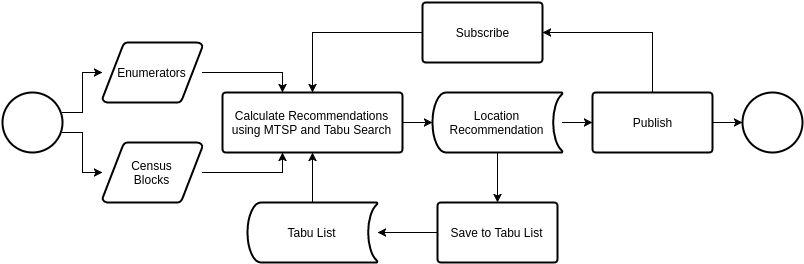
\includegraphics[width=\textwidth]{../../Resources/Images/design_overview}
    \caption{Garis Besar Sistem Usulan}
    \label{fig:design_overview}
\end{figure}


\section{Penyusunan Rekomendasi}

Pada tahap perumusan rekomendasi, input data yang terdiri dari data pencacah dan data blok sensus akan dioleh menjadi rekomendasi path yang harus dikunjungi. Proses penyusunan rekomendasi menggunakan metode \textit{Multiple Travelling Salesman Problem} (MTSP), yang merupakan pengembangan dari metode klasik \textit{Travelling Salesman Problem} (TSP).


Metode MTSP yang digunakan dalam masalah ini memiliki beberapa \textit{requirements}, antara lain:

\begin{itemize}
\item Jumlah \textit{depot} \\
MTSP dapat menggunakan lebih dari satu depot, dengan $ m_{j} $ \textit{salesman} untuk setiap depot $ j $. Pada permasalahan ini menggunakan \textit{non-fixed destination}, sehingga pencacahan tidak perlu kembali ke lokasi dimana pencacahan dimulai.
\item Jumlah \textit{salesman} \\
Jumlah \textit{salesman} yang digunakan dapat berupa \textit{fixed number} $ m $, atau dinamis dengan dibatasi jumlah maksimal $ max(m) $. Pada permasalahan ini digunakan \textit{fixed number} $ m $ pencacah.
\item \textit{Fixed charges} \\
Jika jumlah \textit{salesman} dinamis, maka bisa juga masing-masing \textit{salesman} dibatasi dengan sejumlah biaya tertentu. Pada permasalahan ini tidak digunakan \textit{fixed charges}.
\item Waktu kunjungan (\textit{time windows}) \\
\textit{Time windows} merepresentasikan waktu yang dihabiskan selama kunjugan dalam sebuah \textit{node}. Pada kasus ini \textit{time windows} tidak dapat ditentukan karena tidak tersedianya informasi, sehingga dianggap tidak menggunakan \textit{time windows}.
\end{itemize}


Requirements di atas, secara global dapat disederhanakan dalam tabel-tebel berikut. Tabel \ref{tbl:enumerators_overview} menunjukkan rancangan pencacah beserta koordinat \textit{depot}-nya, sementara Tabel \ref{tbl:census_blocks} menunjukkan rancangan blok sensus beserta koordinat dan \textit{time windows}-nya. Dalam fakta lapangan, jarak antara satu blok sensus dengan blok sensus yang lain tidaklah setara. Bisa jadi secara koordinat memiliki jarak yang berdekatan, tetapi secara akses tidaklah mudah. Untuk itu diperlukan sebuah tabel tambahan, yaitu tabel \textit{cost-matrix}, sebagaimana Tabel \ref{tbl:cost_matrix}. \textit{Cost} yang dimaksud disini adalah segala metrik yang dapat digunakan sebagai penimbang (\textit{weight}), misalnya: biaya, jarak, atau waktu tempuh.


\begin{table}[]
\centering
\caption{Table Pencacah}
\label{tbl:enumerators_overview}
\begin{tabular}{@{}lcc@{}}
\toprule
\multirow{2}{*}{Pencacah} & \multicolumn{2}{l}{\textit{Depot Coordinate}} \\ \cmidrule(l){2-3} 
                          & X                 & Y                \\ \midrule
Pencacah 1                & 20.0              & 20.0             \\
Pencacah 2                & 20.0              & 20.0             \\
Pencacah 3                & 30.0              & 40.0             \\
Pencacah 4                & 30.0              & 40.0             \\
...                       &                   &                  \\
Pencacah m                & x                 & y                \\ \bottomrule
\end{tabular}
\end{table}


\begin{table}[]
\centering
\caption{Tabel Blok Sensus}
\label{tbl:census_blocks}
\begin{tabular}{@{}lccc@{}}
\toprule
\multirow{2}{*}{Blok Sensus} & \multicolumn{2}{c}{Koordinat Lokasi} & \multirow{2}{*}{Time Windows} \\ \cmidrule(lr){2-3}
                             & X                 & Y                &                               \\ \midrule
001B                         & 62.0              & 63.0             & 0                             \\
002B                         & 63.0              & 69.0             & 0                             \\
003B                         & 46.0              & 10.0             & 0                             \\
004B                         & 61.0              & 33.0             & 0                             \\
...                          &                   &                  &                               \\
n                            & x                 & y                & 0                             \\ \bottomrule
\end{tabular}
\end{table}


\begin{table}[]
\centering
\caption{Table \textit{Cost-Matrix}}
\label{tbl:cost_matrix}
\begin{tabular}{@{}|c|c|c|c|c|c|c|@{}}
\toprule
        & 001B & 002B & 003B & 004B & ... & BS ke-n \\ \midrule
001B    & -    & 5    & 2    & 2    &     & ...     \\ \midrule
002B    &      & -    & 4    & 2    &     & ...     \\ \midrule
003B    &      &      & -    & 7    &     & ...     \\ \midrule
004B    &      &      &      & -    &     & ...     \\ \midrule
...     &      &      &      &      & -   & ...     \\ \midrule
BS ke-n &      &      &      &      &     & -       \\ \bottomrule
\end{tabular}
\end{table}


Tabel \textit{cost-matrix}, selain dapat didefinisikan secara manual (berdasarkan hasil survei atau perkiraan \textit{subject matter}), dapat juga didekati dengan menggunakan Google Directions API \citep{google_google_2016}. \textit{Request} yang digunakan menggunakan standar REST API, sementara \textit{response} yang ditampilkan dalam format JSON. Listing \ref{lst:google_direction_api_request} menunjukkan contoh \textit{request}, dan Gambar \ref{fig:google_direction_api_response} menunjukkan contoh \textit{response} dari Google Direction API.








%Gambar \ref{fig:mtsp_solution_example} berikut menunjukkan hasil rekomendasi dengan MTSP.
%
%
%\begin{figure}[h]
%    \centering
%    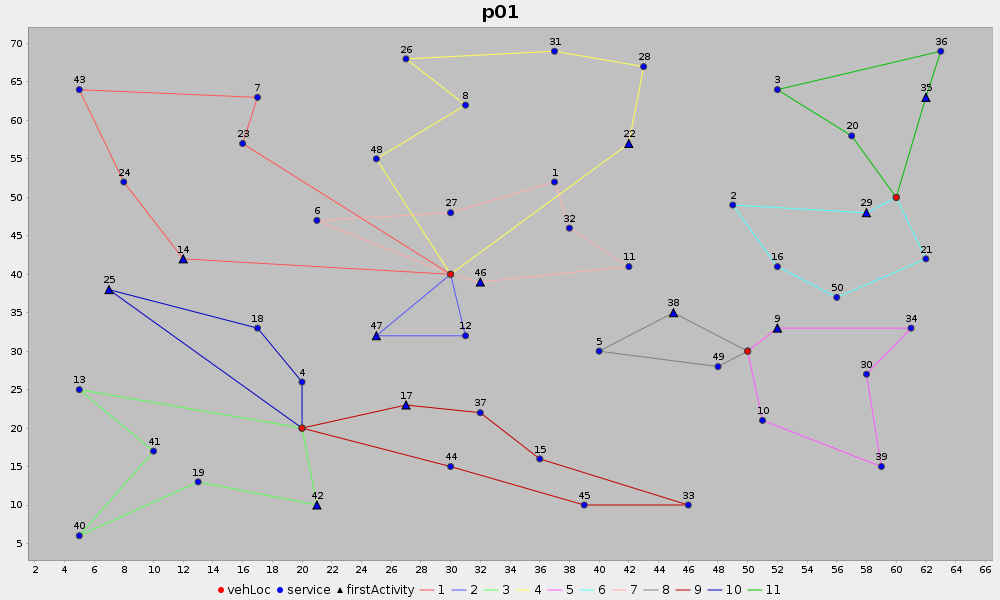
\includegraphics[width=\textwidth]{../../Resources/Images/mtsp_solution_example}
%    \caption{Contoh Hasil Rekomendasi}
%    \label{fig:mtsp_solution_example}
%\end{figure}


\section{Penyusunan \textit{Conflict Resolution}}


\section{\textit{Publish-Subscribe} Rekomendasi}
\end{comment}
%#############################################################################%
